\subsection{Open Loop Control}
	The DoodleBot uses two stepper motors in open loop to control the position and movement of the drawing head (open loop justification in Section~\ref{sec:control-stepper}). The input to the system is the frequency of voltage pulses and the output is the velocity of the drawing head. 
	
	Both the input and output operate in 'step' units (see Section~\ref*{sec:implementation-mechanical} for more detail on what this unit is in the real system).
	
	For this system to operate as required, there are constraints on the maximum acceleration the system can run at.
	
\subsection{Stepper Motors and Open Loop Justification}
		\label{sec:control-stepper}
			
		Stepper Motors are brushless DC motors and are used as the primary drivers for X and Y movement in the DoodleBot. Where a standard DC motor creates an output torque proportional to input current, a stepper motor rotates at a speed that matches the frequency of input voltage steps.
		
		\begin{figure}[h]
			\centering
			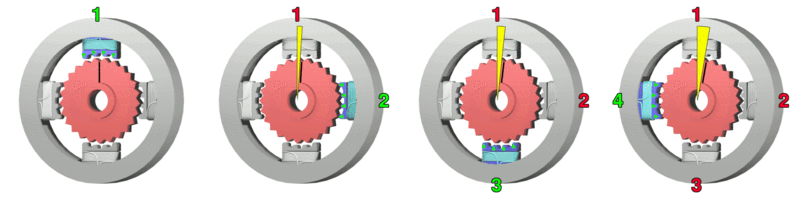
\includegraphics[width=0.8\textwidth]{figures/optimisation/steppermotor}
			\caption[Operation of a simple stepper motor]{Operation of a simplified stepper motor over four steps. \textit{Source: Wapcaplet; Trevolt. Gif of Wapcaplet's 
			4 images. Wikimedia Commons.\cite{website:stepper}}}
			\label{fig:stepper}
		\end{figure}
		
		As shown in Figure~\ref{fig:stepper}, stepper motors consist of several electromagnets arranged in a equally spaced pattern around a gear-shaped rotor. Each electromagnet is shaped to have its own teeth that can align with the rotor's teeth. 
		
		When the stepper motor driver receives a single voltage step, it provides a constant current to the first electromagnet, creating magnetic force that rotates the rotor a small amount (a single step) such that the teeth on the rotor gear align with the teeth on the magnet. Damping in the mechanical system prevent oscillations about this point. As long as the input voltage pulse is maintained, this electromagnet will remain active.
		
		When the first electromagnet is aligned with the rotor teeth, the second electromagnet will be out of alignment. When a second input voltage pulse is received, the stepper motor driver will activate the second electromagnet, causing the rotor to make another rotation step such that it is now in alignment with the second electromagnet. This process continues sequentially across numerous electromagnets around the rotor.
		
		The important thing to note is that the speed of rotation is proportional to the frequency in which the input voltage pulses are received. As long as the magnetic force provided by the electromagnet is enough for the rotor to make the required step within the time the electromagnet is active, the mechanical load on the rotor does not effect the average speed at all. A lighter load may allow the individual step to be quicker, but as the second step will not be made until the next input pulse is received, the differences between a heavy and light load are negligible.
		
		This behaviour means that within certain torque constraints, the stepper motor is a robust and predictable device that we can run in open loop. Since the loads on the system do not vary significantly between possible states (the gravitational force is always the same orientation for all states and mass is constant) the torque constraint can be approximated by an acceleration constraint.